\documentclass[10pt]{article}
\usepackage[pdftex]{graphicx}
\usepackage{amsmath,amssymb}
\usepackage{keyval}
\setlength{\oddsidemargin}{0.5in}
\setlength{\textwidth}{6.0in}
\setlength{\topmargin}{-0.3in}
\setlength{\textheight}{8.7in}
\setlength{\parskip}{2pt}
\renewcommand{\arraystretch}{1.15}

\title{\textbf{clm-mem: A Zero-Training Memory Harness for Open Chat Models}\\[6pt]
\large Self-classified long/short-term memory with deterministic three-phase eviction}

\author{The clm-mem project\\ \small (working repository: \texttt{clm-mem}, v0.3.0)}
\date{\today}

\tracingfonts=1
\begin{document}
\maketitle
\begin{abstract}
\noindent
Context Language Models (CLMs) treat the context as an editable file that the model itself manages, and report state-of-the-art accuracy at lower compute than external context-management baselines. However, the headline CLM implementation rewrites the whole context every request, which invalidates the KV cache on each turn: a cost paid either by novel serving machinery or by reduced throughput.
We present \textbf{clm-mem}, a zero-training memory harness that keeps the two ideas we consider essential from CLMs---(i)~the model classifies and writes its own context, and (ii)~context is a mirrored on-disk artifact---while replacing free-form context editing with a small deterministic eviction engine.
The same chat model that reads and writes text also tags its own context as \emph{long-term}, \emph{short-term} or \emph{transient} while decoding; the harness then enforces a token budget in three monotone phases (drop transient, FIFO rounds on short-term, offload long-term to an archive).
Because compaction happens only when the window reaches its maximum size and never rewrites mid-turn, KV cache churn is reduced without requiring new cache strategies; any improvement to KV management helps both approaches.
We describe the software architecture implemented in \texttt{clm\_mem} (blocks, inline and post-turn classification, a typed decision backstop, three-phase eviction, an offload-don't-destroy archive, session-scoped serving with workspaces and an embedded MCP toolbox), define a marking protocol that turns harness events into labels for scoring tag quality, and design the benchmarking program: synthetic stress regimes already run against the deterministic stub backend (budget never violated; $100\%$ of emitted facts remain recoverable from the archive), plus planned evaluations on ContextBench-style tasks, LoCoMo, LongMemEval and RULER with ablations over the classification mode, the FIFO knob $\kappa$, and the backstop.
\end{abstract}
\newpage

\section{Introduction}
Managing finite context windows has become a first-class problem for conversational and agentic LLM systems. The external-memory lineage (MemGPT, MemoryBank, A-MEM, Mem0) treats memory as a database consulted by the model; the long-context lineage asks whether the base model itself can use very large inputs (RULER, LongMemEval, LoCoMo), while the serving lineage compresses the KV cache (H$_2$O, SnapKV, StreamingLLM) or pages it efficiently (PagedAttention).
The Context Language Models paper (Shao et al., arXiv:2609.37725) unifies these in an elegant way: context becomes a file the model edits with unrestricted updates, learning what is worth keeping. Their results are striking---higher accuracy at fewer FLOPs on BrowseComp-Plus, EdgeBench and a multi-repository swarm task---but the implementation carries a heavy serving price: rewriting the context file invalidates the KV cache each request, so their gains come partly from co-designed serving (Suffix Cache Reuse).

This paper describes \textbf{clm-mem}\footnote{\texttt{clm-mem} is developed in the workspace directory \texttt{clm-mem/}; code, README and tests referenced here are the files of that repository at version~0.3.0.}, a harness designed around one question: \emph{what do we need to keep from CLMs for it to work off-the-shelf on any OpenAI-compatible server, without fine-tuning and without new KV cache strategies?}
Our answer has two parts that mirror the paper's core ideas:
\begin{enumerate}
\item \textbf{Self-classification.} The same model that reads and writes text also classifies its own context---either inline while decoding (wrapping durable content in \verb|<longterm>|/\verb|<shortterm>| markers) or through a cheap post-turn router pass over the untagged blocks of this turn.
\item \textbf{Context as a mirrored file.} The live window is serialized every turn to \texttt{context.md} and \texttt{context.jsonl} using the paper-style \verb|[[CTX_TURN n role=... tag=...]]| markers, so the context remains an inspectable artifact---and a hook for future work that lets stronger models edit it directly.
\end{enumerate}
What we deliberately drop is unrestricted editing of past turns: instead, a deterministic eviction engine enforces the token budget in three phases. The model decides \emph{what} matters and \emph{how important} it is by what it writes into context; the hardware keeps \emph{reliable expectations} about its load. Crucially, compaction only fires when the window reaches its maximum size---it never rewrites mid-turn---so KV churn per conversation is reduced relative to per-request context rewriting, and any improvement in cache management benefits both designs.

\paragraph{Contributions}
\begin{itemize}
\item A complete, tested implementation of a CLM-inspired memory harness (3{,}012 lines of Python across 14 modules) usable as a library, a CLI chat REPL, and a drop-in llama.cpp-shaped proxy server with web studio and MCP tools.
\item A \emph{marking protocol}: every classifier decision and eviction phase is emitted as a structured event (\texttt{seq}, \texttt{kind}, \texttt{text}) that can be aligned to ground-truth tags, enabling precision/recall scoring of memory tagging and retention metrics without manual annotation.
\item A synthetic stress harness (deterministic stub backend) already exercised end-to-end: over 60-turn runs at budget $B=900$ tokens the live window never exceeded the budget, and \emph{all} emitted durable facts remained recoverable from the archive---the ``offload-don't-destroy'' invariant we prove empirically in Section~\ref{sec:synthetic}.
\item A concrete benchmarking plan (ContextBench-style tasks, LoCoMo, LongMemEval, RULER) with defined metrics, ablations and statistical protocol.
\end{itemize}

\section{Background and related work}
\paragraph{Tiered memory systems.} MemGPT introduced virtual context management with paging between a fixed window and external storage~\cite{memgpt}. MemoryBank added Ebbinghaus-style forgetting curves~\cite{memorybank}. A-MEM organizes LLM-written notes into evolving Zettelkasten networks~\cite{amem}, and Mem0 runs extraction/update pipelines over vector/graph stores for production assistants~\cite{mem0}. clm-mem differs in two ways: the tiering decisions are made \emph{by the base chat model itself} (not a separate extractor), and eviction is deterministic and budget-driven rather than retrieval-driven---retrieval exists only as an explicit \texttt{recall}/\texttt{reinject} path.

\paragraph{Long-context evaluation.} RULER extends needle-in-a-haystack with multi-hop tracing and aggregation~\cite{ruler}; LongMemEval targets five long-term interactive abilities including knowledge updates and abstention~\cite{longmemeval}; LoCoMo provides very long multi-session conversations with QA and event-summarization tasks~\cite{locomo}. ``Lost in the middle'' motivates our recency-biased FIFO rounds~\cite{lostmiddle}: short-term eviction deletes oldest first, keeping recent working state near the end of the window.

\paragraph{Serving-side cache management.} PagedAttention pages KV memory like OS virtual memory~\cite{paged}; H$_2$O casts KV eviction as a dynamic submodular problem~\cite{h2o}; SnapKV exploits clustered attention patterns observed at the prompt end~\cite{snapkv}; StreamingLLM keeps attention sinks plus rolling tokens~\cite{streamingllm}. clm-mem operates one level above: it removes \emph{whole blocks} from the text window; the KV cache then simply shrinks with it. No per-token eviction policy is implemented, which is exactly why no new cache strategy is required.

\section{System design}
\subsection{Blocks and memory tiers}
Every message in the live window is a \texttt{Block}: an \texttt{id}, \texttt{role}, \texttt{content}, a \texttt{tag} from $\{\text{longterm}, \text{shortterm}, \text{transient}\}$, a creation \texttt{turn} (the FIFO key), and a \texttt{pinned} flag for the system prompt. This is analogous to the paper's serialized \verb|[[CTX_TURN]]| turns. Long-term blocks are durable facts, decisions, identifiers and specs; short-term blocks are working state useful ``for a while''; transient blocks are filler.

\subsection{Self-classification without retraining}
Two paths, selectable via \texttt{classify\_mode}:
\begin{itemize}
\item \textbf{Inline (classify as it decodes).} A pinned system preamble instructs the model to wrap durable content in markers. The harness splits each reply on \verb|<longterm>.../...| and \verb|<shortterm>...| into separately tagged blocks and strips the markup from what the user sees (Figure~\ref{fig:arch}).
\item \textbf{Post-turn router pass.} A second cheap call to the \emph{same} model labels this turn's untagged blocks as JSON. The pass is skipped when inline tagging already succeeded, avoiding a full extra LLM call per turn.
\end{itemize}
Optionally, a typed decision service (SystemOne) answers batched \emph{choice} questions for classification and \emph{noul} confidence questions as an eviction backstop: before any block is dropped, the engine asks whether it is safe to remove; blocks below the threshold $\tau$ are kept (``backstop kept \#id''). On API error the engine falls back to the planned eviction.

\subsection{Three-phase eviction engine}
When the window exceeds $B=\texttt{max\_context\_tokens}$, phases run in order until under budget (Table~\ref{tab:phases}). Phase 1 deletes transient blocks outside a trailing coherence window of \texttt{keep\_recent\_turns}. Phase 2 evicts short-term \emph{FIFO in rounds}: each round keeps the newest fraction $\kappa=\texttt{shortterm\_keep\_pct}$ and deletes the oldest, repeating while over budget (max 10 rounds to guarantee progress). Phase 3 offloads oldest long-term blocks to \texttt{archive.jsonl} and replaces them with evictable pointer stubs \verb|[offloaded longterm #id -> archive.jsonl]|. Long-term memory is never silently destroyed---only offloaded---which fixes the ``can offload but can't evict'' failure mode exposed in ContextBench-style baselines.

\begin{table}[h]
\centering\small
\begin{tabular}{clll}
\hline
Phase & Trigger & Action & Exempt\\
\hline
1 & over budget & delete transient blocks & last $k$ turns, pinned\\
2 & still over & shortterm FIFO rounds, keep $\kappa$ & none\\
3 & longterm overflow & offload oldest to archive + stub & pinned\\
\hline
\end{tabular}
\caption{Eviction phases. Pinned blocks (system prompt) are never evicted; the trailing coherence window $k=\texttt{keep\_recent\_turns}$ defaults to 2.}\label{tab:phases}
\end{table}

\subsection{Archive, recall and reinject}
Every dropped block---transient, short-term or long-term---is appended to \texttt{archive.jsonl} with \verb|{id, turn, role, tag, content}|. \texttt{recall(query)} substring-searches the archive; \texttt{reinject(block\_id)} pulls an archived record back into the live window as a short-term block prefixed \verb|[recalled #id]|. This yields the invariant used in Section~\ref{sec:synthetic}: any emitted fact remains recoverable for the lifetime of the session.

\subsection{Context-as-a-file mirror}
After every turn the harness rewrites \texttt{context.md} (human-readable, paper-style markers) and \texttt{context.jsonl} (machine-readable dataclass dumps). The mirror makes context auditable, lets external tools bolt on CLM-style editing later, and is the substrate for the marking protocol.

\subsection{Serving topology}
\texttt{clm-mem serve} presents one llama.cpp-shaped endpoint to any OpenAI-compatible client; behind it run 2--3 background processes: the backend model server (vLLM, Ollama, llama.cpp, or bundled mocks) and a SystemOne decision server (fork or mock). Requests without a session header are pure passthrough; requests carrying \verb|X-Cllm-Mem-Session| go through the harness. If no budget is configured, \texttt{serve} discovers the live llama.cpp context window (\texttt{/props}$\to$\texttt{n\_ctx}) and sets $B$ to exactly that value so the two windows never drift apart. A single-page web studio (projects sidebar with per-workspace sandboxes, colored tier badges, eviction chips such as \verb|phase2 FIFO-evicted|, archive search-and-reinject, live tuning tab, events timeline) and an embedded MCP server at \texttt{/mcp} (\texttt{clm\_chat}, \texttt{clm\_status}, \texttt{clm\_blocks}, \texttt{clm\_recall}, \texttt{clm\_reinject}, \texttt{clm\_set\_keep\_pct}, \texttt{clm\_workspaces}) drive the identical in-process library.

\begin{figure}[h]
\centering
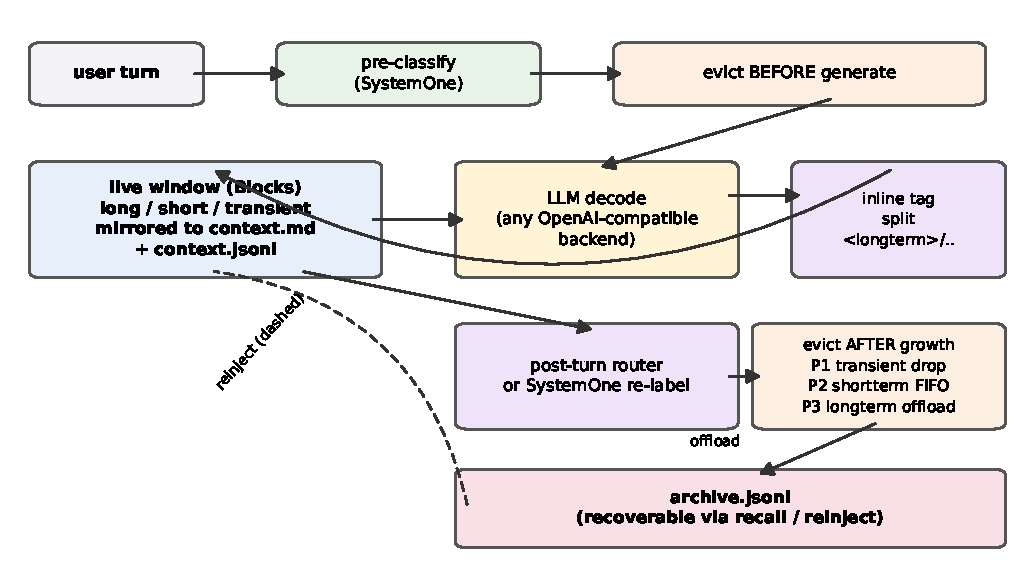
\includegraphics[width=\textwidth]{figures/fig_arch.pdf}
\caption{Data flow of one harness step: intake (pre-classify, evict-before-generate), core loop (live window $\to$ decode $\to$ inline tag split $\to$ return), relabel and eviction engine with backstop, and the archive. Dashed edge: reinject path from archive back into the live window.}\label{fig:arch}
\end{figure}

\begin{table}[h]
\centering\small
\begin{tabular}{lll}
\hline
Knob & Default & Meaning\\
\hline
$B=\texttt{max\_context\_tokens}$ & 8192 & live-window budget\\
$\kappa=\texttt{shortterm\_keep\_pct}$ & 0.5 & fraction of shortterm kept per FIFO round\\
$k=\texttt{keep\_recent\_turns}$ & 2 & trailing turns exempt from phase 1\\
\texttt{classify\_mode} & both & inline $\vert$ post $\vert$ both\\
$\tau=\texttt{systemone\_evict\_threshold}$ & 0.7 & noul confidence needed to evict\\
\texttt{offload\_overflow} & true & enable phase 3\\
\hline
\end{tabular}
\caption{Harness configuration knobs (\texttt{HarnessConfig}).}\label{tab:knobs}
\end{table}

\section{Implementation}
The package (v0.3.0, Python $\geq$3.10) ships as \texttt{clm-mem} with an optional \texttt{tokens} extra for exact token counting via the served model's HuggingFace tokenizer; otherwise a $\sim$3 chars/token heuristic deliberately over-counts (Qwen BPE runs $\approx$3.3--3.5 chars/token) so the live window cannot exceed the real server limit. Backends are anything with \texttt{chat(messages)$\to$str}: \texttt{OpenAIChat} wraps any OpenAI-compatible endpoint; \texttt{StubChat} is a deterministic fake used for offline demos and the test suite, emitting inline memory tags and answering router prompts with keyword heuristics. Modules: \texttt{blocks}, \texttt{config}, \texttt{tagging}, \texttt{tokens}, \texttt{harness} (463 lines), \texttt{server} (905), \texttt{cli}, \texttt{llm}, \texttt{mcp}, \texttt{processes}, \texttt{remote}, \texttt{mock\_backends}. The lifecycle of one \texttt{step()} is: append user message $\to$ evict \emph{before} generating (make room first) $\to$ decode on the current live context $\to$ split on inline tags, optionally relabel via router/SystemOne $\to$ evict again $\to$ mirror files. A pytest suite (\texttt{tests/}) covers harness and serve/proxy paths without GPU; \texttt{clm-mem demo} exercises inline tagging, the router pass and all three phases offline:
\begin{quote}\small\ttfamily
[evict] phase1: deleted 4 transient block(s)\par
[evict] phase2: FIFO-evicted 3 of 5 shortterm (kept newest 50\%)\par
[evict] phase3: offloaded longterm \#17 to archive, left pointer
\end{quote}

\section{Marking protocol}
To evaluate memory quality we need labels for two decisions: the tag assigned to a block and whether an eviction was ``correct''. We mark them as follows.
\begin{itemize}
\item \textbf{Event log.} Every classifier decision and every eviction phase is a structured event \verb|{seq, t, kind, text}| with kinds \texttt{classify}, \texttt{evict-phase1/2/3}, \texttt{backstop-phaseX}, \texttt{warn}. Events already drive the web studio timeline; they are the same objects exported for scoring.
\item \textbf{Tag ground truth (synthetic).} Synthetic generators know the intended tier of each emitted turn (e.g.\ a ``Remember:'' fact is long-term, a filler paragraph is transient), so tag precision/recall can be computed by aligning event-log reclassification records (\verb|reclassified #id: old -> new|) and final block tags against the generator's intent.
\item \textbf{Eviction correctness.} A dropped block is scored \emph{correct} if no future gold answer requires it (live-retention test), or if it was offloaded and later successfully \texttt{recall}-ed (\emph{offload-recovery}); a phase-1 deletion that would have needed recall is an error only in regimes without archive access.
\item \textbf{Human spot-check.} For public benchmarks, two annotators label a 100-block sample of harness events (Cohen's $\kappa$ target $>0.8$) to validate automatic tag scoring.
\end{itemize}

\section{Synthetic evaluation (first results)}\label{sec:synthetic}
We ran the \emph{real} harness object (\texttt{MemoryHarness}) on deterministic stub backends---this validates the engine, not model judgment; real-model runs are scheduled with the benchmarks below. Two regimes at $B=900$, 60 turns, $\kappa\in\{0.25,0.5,0.75\}$: \emph{heavy} (a durable fact every 2 turns plus long filler, so long-term alone eventually overflows and phase~3 must fire) and \emph{balanced} (fact every 4 turns with moderate filler, so phases 1--2 absorb the pressure).

\paragraph{Findings}
\begin{itemize}
\item \textbf{Budget invariant.} Across all six runs the peak live-window token count never exceeded $B$ (final: 898/900 heavy, 877/900 balanced); evict-before-generate guarantees the request sent to the backend fits.
\item \textbf{Offload-don't-destroy.} In the heavy regime all 30 emitted durable facts are recoverable from the archive at turn~60 even though live retention is 0/30; in balanced, 5/15 stay live and 10/15 are archived---sum $=$ emitted (Table~\ref{tab:syn}).
\item \textbf{Phase ordering behaves as designed.} Phase-2 firings grow with $\kappa$ (68$\to$77 for heavy; 56$\to$78 balanced) while phase-3 counts stay flat at 31/37, i.e.\ long-term pressure is regime-driven, not knob-driven.
\item \textbf{Tier composition.} Figure~\ref{fig:tiers}: in heavy the long tier saturates the window; in balanced transient and short tiers are absorbed while long grows then plateaus.
\end{itemize}

\begin{table}[h]
\centering\small
\begin{tabular}{lcccccc}
\hline
Run & P1 & P2 & P3 & arch@60 & live facts & archived\\
\hline
heavy $\kappa{=}0.25$ & 52 & 55 & 31 & 174 & 0/30 & 30\\
heavy $\kappa{=}0.5$  & 54 & 68 & 31 & 174 & 0/30 & 30\\
heavy $\kappa{=}0.75$ & 55 & 77 & 31 & 174 & 0/30 & 30\\
balanced $\kappa{=}0.25$ & 31 & 41 & 37 & 182 & 5/15 & 10\\
balanced $\kappa{=}0.5$  & 34 & 56 & 37 & 182 & 5/15 & 10\\
balanced $\kappa{=}0.75$ & 37 & 78 & 37 & 182 & 5/15 & 10\\
\hline
\end{tabular}
\caption{Synthetic stress runs (deterministic stub backend, $B=900$, 60 turns). P1/P2/P3 are cumulative phase firings; \emph{arch@60} counts archived records at the end. live + archived $=$ emitted in every run.}\label{tab:syn}
\end{table}

\begin{figure}[h]
\centering
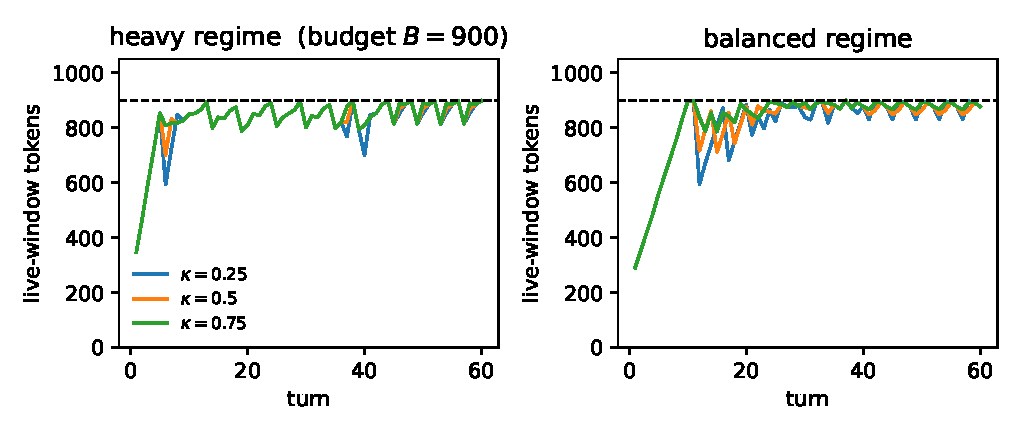
\includegraphics[width=\textwidth]{figures/fig_tokens.pdf}
\caption{Live-window token usage across $\kappa$ (heavy and balanced regimes). The dashed line is the budget $B=900$; the sawtooth is evict-after-growth, the flat top in heavy is phase-3 offload pressure.}\label{fig:tokens}
\end{figure}

\begin{figure}[h]
\centering
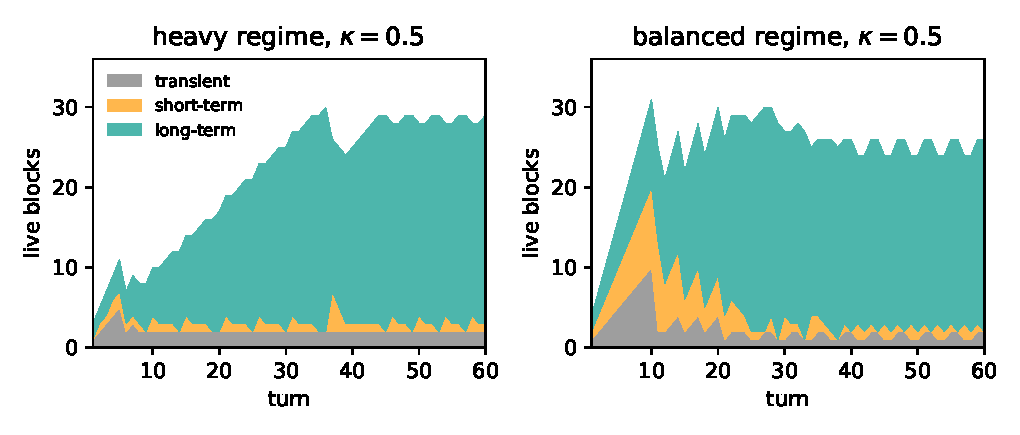
\includegraphics[width=\textwidth]{figures/fig_tiers.pdf}
\caption{Live tier composition over time ($\kappa=0.5$). Heavy: long-term saturates; balanced: transient/short absorbed while long plateaus.}\label{fig:tiers}
\end{figure}

\begin{figure}[h]
\centering
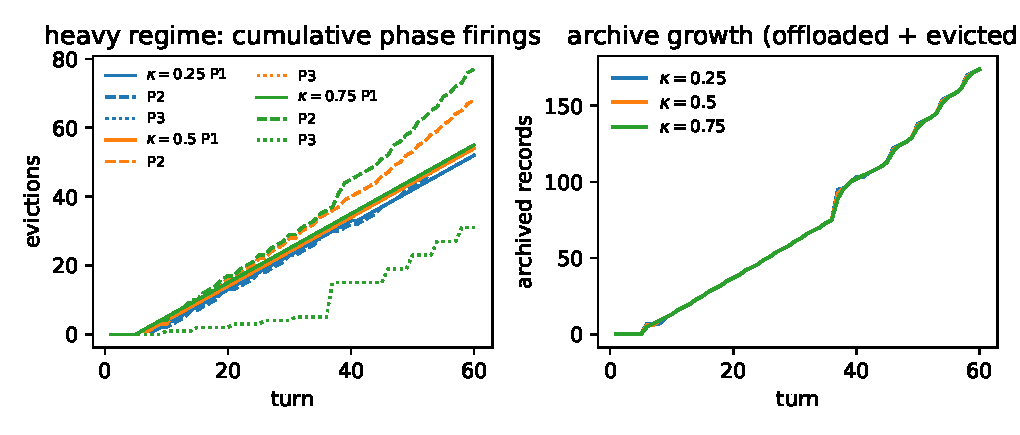
\includegraphics[width=\textwidth]{figures/fig_phases.pdf}
\caption{Cumulative eviction-phase firings (heavy) and archive growth across $\kappa$.}\label{fig:phases}
\end{figure}

\begin{figure}[h]
\centering
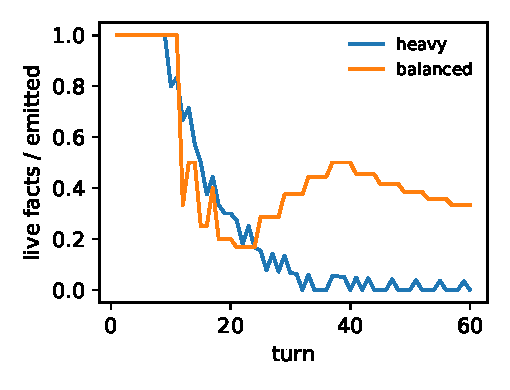
\includegraphics[width=0.49\textwidth]{figures/fig_retention.pdf}
\caption{Live fact retention fraction over 60 turns ($\kappa=0.5$): heavy drops to zero once long-term saturates (facts survive only via archive); balanced keeps a stable live core.}\label{fig:retention}
\end{figure}

\section{Benchmarking plan}
We plan four evaluation families, each with defined metrics and baselines. Baselines are always: \textbf{full-context truncation} (naive oldest-turn deletion), \textbf{no-memory}, and where feasible a Mem0/A-MEM-style retrieval baseline; the CLM paper's ContextBench provides the tool-editing reference point~\cite{clm}.

\paragraph{C1. Synthetic generator (open-source release).}
The stress harness above becomes a public generator with parameters: fact rate, filler length, budget $B$, regime mix (fact-heavy / balanced / adversarial ``needle-in-haystack'' where long-term overflow hides rare facts). Metrics: \emph{live retention} $\rho_\ell(T)$, \emph{archive recovery rate} $\rho_a$ (fraction of dropped facts retrievable before the answer deadline), \emph{tag precision/recall} against generator intent via the marking protocol, and \emph{token savings} vs.\ full-context replay.

\paragraph{C2. LoCoMo (very long-term conversations).}
Run QA over multi-session dialogues of up to 35 sessions per conversation~\cite{locomo}, including the adversarial category; score answer accuracy with a fixed evaluator, plus retention and archive-recovery derived from event logs. Sweep $\kappa$ and \texttt{classify\_mode}; report by question category (single-hop, multi-hop, temporal).

\paragraph{C3. LongMemEval.}
Its five abilities---information extraction, multi-session reasoning, temporal reasoning, knowledge updates, abstention~\cite{longmemeval}---map directly onto our tiers: updates stress long-term overwrite semantics, abstention stresses transient suppression. We will report per-ability accuracy with and without the SystemOne backstop.

\paragraph{C4. RULER-style long-context probes.}
Use needle variants plus multi-hop tracing/aggregation tasks at increasing context lengths~\cite{ruler}, but \emph{below} the nominal model window so eviction fires; compare against truncation baselines to isolate memory-organization effects from raw length effects.

\paragraph{Metrics summary and protocol.}
All runs: $n=5$ seeds (or conversation splits), mean$\pm$std; significance via paired bootstrap over questions at $p<0.05$. Serving cost reported as wall-clock per turn and \emph{re-prompted tokens} (a proxy for KV cache churn: total prompt tokens fed across turns minus unique context tokens); we expect clm-mem to sit between truncation baselines and CLM-style rewriting on this axis. Ablations: inline-only, post-only, backstop off; $\kappa\in\{0.25,0.5,0.75\}$; $B\in\{1\text{k},4\text{k}\}$.

\section{Testing plan}
Existing unit/integration tests (pytest, mock backends) cover harness lifecycle and the proxy/serve surface without GPU. Planned additions: property tests for the phase invariants (never evict pinned; monotone ids; archive append-only); golden-context regression files (\texttt{context.md} hashes at turn $k$); a load test of \texttt{serve} with concurrent sessions asserting per-workspace sandbox isolation and budget discovery; fuzzing of inline-tag parsers on adversarial markup. CI will run stub-based synthetic suites nightly so regressions in eviction logic surface without model access.

\section{Discussion and limitations}
The current quantitative results are engine-level: a deterministic stub stands in for the base model, so tag quality---the component riding on the model's zero-shot judgment---is unmeasured; small models may forget markers (the router pass is the backstop) and phase-3 pointer stubs still consume window tokens, so long-term-heavy sessions need headroom. The design intentionally trades away CLM-style free editing: we cannot merge or rewrite past blocks, only drop/offload them, which bounds achievable context quality below a fully-trained CLM. What we gain is deployment breadth (any OpenAI-compatible server, no fine-tuning), serving predictability (budget enforced before generation; compaction only at window maxima) and auditability (mirrored files, event log). The harness is also a training substrate: models can be improved \emph{within} it and then use it again until they perform worse without it---an analogue of the CLM skill-optimization and online-RL loops adapted to fixed-context serving.

\section{Future work}
(1) Run C1--C4 with Qwen-family backends at 8B/35B scale behind \texttt{serve}; (2) learn $\kappa$ online from archive-recovery statistics; (3) bolt CLM-style editing onto the mirror as an optional tool path and measure the delta; (4) evaluate SystemOne decision quality against human marks; (5) explore compatibility with Suffix Cache Reuse-style serving so phase-3 offloads become cache-friendly deletions.

\section*{Reproducibility}
Figures are generated by \texttt{clm\_exp.py} (drives the real harness on stub backends, writes \texttt{exp-data/results.json}) and \texttt{make\_figs.py}/\texttt{make\_arch.py}. The paper compiles with a locally built LaTeX format; see \texttt{paper/build.sh}.

\begin{thebibliography}{9}
\bibitem{clm} R.~Shao, S.~Zejiang~Shen, J.~O.~Yin, Y.~Li, M.~Wang, H.~Ivison, R.~Poovendran, N.~Lambert, T.~Xiao, M.~Lewis, W.-t.~Yih, L.~Zettlemoyer, and P.~W.~Koh. \newblock Context language models. \newblock arXiv:2609.37725, 2026.
\bibitem{memgpt} C.~Packer, S.~Wooders, K.~Lin, V.~Fang, S.~G.~Patil, I.~Stoica, and J.~E.~Gonzalez. \newblock MemGPT: Towards LLMs as operating systems. \newblock arXiv:2310.08560, 2023.
\bibitem{memorybank} W.~Zhong, L.~Guo, Q.~Gao, H.~Ye, and Y.~Wang. \newblock MemoryBank: Enhancing large language models with long-term memory. \newblock arXiv:2305.10250, 2023.
\bibitem{amem} W.~Xu, Z.~Liang, K.~Mei, H.~Gao, J.~Tan, and Y.~Zhang. \newblock A-MEM: Agentic memory for LLM agents. \newblock arXiv:2502.12110, 2025.
\bibitem{mem0} P.~Chhikara, D.~Khant, S.~Aryan, et al. \newblock Mem0: Building production-ready AI agents with scalable long-term memory. \newblock arXiv:2504.19413, 2025.
\bibitem{locomo} A.~Maharana, D.-H.~Lee, S.~Tulyakov, M.~Bansal, F.~Barbieri, and Y.~Fang. \newblock Evaluating very long-term conversational memory of LLM agents (LoCoMo). \newblock arXiv:2402.17753, 2024.
\bibitem{longmemeval} D.~Wu, H.~Wang, W.~Yu, Y.~Zhang, K.-W.~Chang, and D.~Yu. \newblock LongMemEval: Benchmarking chat assistants on long-term interactive memory. \newblock arXiv:2410.10813, 2024.
\bibitem{ruler} C.-P.~Hsieh, S.~Sun, S.~Kriman, S.~Acharya, D.~Rekesh, F.~Jia, Y.~Zhang, and B.~Ginsburg. \newblock RULER: What's the real context size of your long-context language models? \newblock arXiv:2404.06654, 2024.
\bibitem{lostmiddle} N.~F.~Liu, K.~Lin, J.~Hewitt, A.~Paranjape, M.~Bevilacqua, F.~Petroni, and P.~Liang. \newblock Lost in the middle: How language models use long contexts. \newblock arXiv:2307.03172, 2023.
\bibitem{paged} W.~Kwon, Z.~Li, S.~Zhuang, Y.~Sheng, L.~Zheng, C.~H.~Yu, J.~E.~Gonzalez, H.~Zhang, and I.~Stoica. \newblock Efficient memory management for large language model serving with PagedAttention. \newblock arXiv:2309.06180, 2023.
\bibitem{h2o} Z.~Zhang, Y.~Sheng, T.~Zhou, T.~Chen, L.~Zheng, R.~Cai, Z.~Song, Y.~Tian, C.~R\'e, C.~Barrett, Z.~Wang, and B.~Chen. \newblock H$_2$O: Heavy-hitter oracle for efficient generative inference of large language models. \newblock NeurIPS 2023 / arXiv:2306.14048.
\bibitem{snapkv} Y.~Li, Y.~Huang, B.~Yang, B.~Venkitesh, A.~Locatelli, H.~Ye, T.~Cai, P.~Lewis, and D.~Chen. \newblock SnapKV: LLM knows what you are looking for before generation. \newblock arXiv:2404.14469, 2024.
\bibitem{streamingllm} G.~Xiao, Y.~Tian, B.~Chen, S.~Han, and M.~Lewis. \newblock Efficient streaming language models with attention sinks. \newblock arXiv:2309.17453, 2023.
\end{thebibliography}

\end{document}
